% Template for Elsevier CRC journal article
% version 1.2 dated 09 May 2011

% This file (c) 2009-2011 Elsevier Ltd.  Modifications may be freely made,
% provided the edited file is saved under a different name

% This file contains modifications for Procedia CIRP

% Changes since version 1.1
% - added "procedia" option compliant with ecrc.sty version 1.2a
%   (makes the layout approximately the same as the Word CRC template)
% - added example for generating copyright line in abstract

%-----------------------------------------------------------------------------------

%% This template uses the elsarticle.cls document class and the extension package ecrc.sty
%% For full documentation on usage of elsarticle.cls, consult the documentation "elsdoc.pdf"
%% Further resources available at http://www.elsevier.com/latex

%-----------------------------------------------------------------------------------

%%%%%%%%%%%%%%%%%%%%%%%%%%%%%%%%%%%%%%%%%%%%%%%%%%%%%%%%%%%%%%
%%%%%%%%%%%%%%%%%%%%%%%%%%%%%%%%%%%%%%%%%%%%%%%%%%%%%%%%%%%%%%
%%                                                          %%
%% Important note on usage                                  %%
%% -----------------------                                  %%
%% This file should normally be compiled with PDFLaTeX      %%
%% Using standard LaTeX should work but may produce clashes %%
%%                                                          %%
%%%%%%%%%%%%%%%%%%%%%%%%%%%%%%%%%%%%%%%%%%%%%%%%%%%%%%%%%%%%%%
%%%%%%%%%%%%%%%%%%%%%%%%%%%%%%%%%%%%%%%%%%%%%%%%%%%%%%%%%%%%%%

%% The '3p' and 'times' class options of elsarticle are used for Elsevier CRC
%% The 'procedia' option causes ecrc to approximate to the Word template
\documentclass[3p,times,procedia,twocolumn,twoside]{elsarticle}
\flushbottom

%% The `ecrc' package must be called to make the CRC functionality available
\usepackage{ecrc,stfloats}
%\usepackage{amsmath}


%% The ecrc package defines commands needed for running heads and logos.
%% For running heads, you can set the journal name, the volume, the starting page and the authors

%% set the volume if you know. Otherwise `00'
\volume{00}

%% set the starting page if not 1
\firstpage{1}

%% Give the name of the journal
\journalname{Procedia CIRP}

%% Give the author list to appear in the running head
%% Example \runauth{C.V. Radhakrishnan et al.}
\runauth{Author name}

%% The choice of journal logo is determined by the \jid and \jnltitlelogo commands.
%% A user-supplied logo with the name <\jid>logo.pdf will be inserted if present.
%% e.g. if \jid{yspmi} the system will look for a file yspmilogo.pdf
%% Otherwise the content of \jnltitlelogo will be set between horizontal lines as a default logo

%% Give the abbreviation of the Journal.
\jid{cirp}

%% Give a short journal name for the dummy logo (if needed)
%\jnltitlelogo{Procedia CIRP}

%% Hereafter the template follows `elsarticle'.
%% For more details see the existing template files elsarticle-template-harv.tex and elsarticle-template-num.tex.

%% Elsevier CRC generally uses a numbered reference style
%% For this, the conventions of elsarticle-template-num.tex should be followed (included below)
%% If using BibTeX, use the style file elsarticle-num.bst

%% End of ecrc-specific commands
%%%%%%%%%%%%%%%%%%%%%%%%%%%%%%%%%%%%%%%%%%%%%%%%%%%%%%%%%%%%%%%%%%%%%%%%%%

%% The amssymb package provides various useful mathematical symbols

\usepackage{amssymb}
\usepackage{gensymb}
\usepackage{amsmath}

%% The amsthm package provides extended theorem environments
%% \usepackage{amsthm}

%% The lineno packages adds line numbers. Start line numbering with
%% \begin{linenumbers}, end it with \end{linenumbers}. Or switch it on
%% for the whole article with \linenumbers after \end{frontmatter}.
%% \usepackage{lineno}

%% natbib.sty is loaded by default. However, natbib options can be
%% provided with \biboptions{...} command. Following options are
%% valid:

%%   round  -  round parentheses are used (default)
%%   square -  square brackets are used   [option]
%%   curly  -  curly braces are used      {option}
%%   angle  -  angle brackets are used    <option>
%%   semicolon  -  multiple citations separated by semi-colon
%%   colon  - same as semicolon, an earlier confusion
%%   comma  -  separated by comma
%%   numbers-  selects numerical citations
%%   super  -  numerical citations as superscripts
%%   sort   -  sorts multiple citations according to order in ref. list
%%   sort&compress   -  like sort, but also compresses numerical citations
%%   compress - compresses without sorting
%%
\biboptions{sort&compress}

% \biboptions{}

% if you have landscape tables
\usepackage[figuresright]{rotating}
\usepackage{hyperref}
%\usepackage{harvard}
% put your own definitions here:x
%   \newcommand{\cZ}{\cal{Z}}
%   \newtheorem{def}{Definition}[section]
%   ...

% add words to TeX's hyphenation exception list
%\hyphenation{author another created financial paper re-commend-ed Post-Script}

% declarations for front matter
\usepackage{fleqn}
\mathindent0pt
\parskip0pt
\begin{document}

\begin{frontmatter}

%% Title, authors and addresses

%% use the tnoteref command within \title for footnotes;
%% use the tnotetext command for the associated footnote;
%% use the fnref command within \author or \address for footnotes;
%% use the fntext command for the associated footnote;
%% use the corref command within \author for corresponding author footnotes;
%% use the cortext command for the associated footnote;
%% use the ead command for the email address,
%% and the form \ead[url] for the home page:
%%
%% \title{Title\tnoteref{label1}}
%% \tnotetext[label1]{}
%% \author{Name\corref{cor1}\fnref{label2}}
%% \ead{email address}
%% \ead[url]{home page}
%% \fntext[label2]{}
%% \cortext[cor1]{}
%% \address{Address\fnref{label3}}
%% \fntext[label3]{}

\dochead{10th CIRP Conference on Industrial Product-Service Systems, IPS$^{2}$ 2018, 29-31 May 2018,\\ Link\"oping, Sweden}
%% Use \dochead if there is an article header, e.g. \dochead{Short communication}
%% \dochead can also be used to include a conference title, if directed by the editors
%% e.g. \dochead{17th International Conference on Dynamical Processes in Excited States of Solids}

\title{Data based optimization of the operation of industrial chillers}

%% use optional labels to link authors explicitly to addresses:
%% \author[label1,label2]{<author name>}
%% \address[label1]{<address>}
%% \address[label2]{<address>}



\author[a,*]{Benjamin M\"orzinger}
\author[a]{Christoph Loschan}
\author[a]{Florian Kloibhofer}
\author[a]{Friedrich Bleicher}

\address[a]{Institute for Production Engineering and Laser Technology, TU Wien, Getreidemarkt 9, Vienna, 1060, Austria}

\begin{abstract}
In the following paper, we present a novel method for the optimization of operation strategies in the field of production engineering. The balanced manufacturing method uses monitoring data and technical specification documents in order to create a simulation model (virtual twin) and derive optimal operation strategies based on the behaviour of this model. The method is illustrated using a use case. In this use case, industrial chillers where modelled and optimal operation strategies where derived based on multi-criteria optimization. The expected savings in the means of overall energy efficiency are between 15-40\%, while no additional hardware had to be deployed. 
\end{abstract}

\begin{keyword}
Optimization; Simulation; Chillers

%% keywords here, in the form: keyword \sep keyword

%% PACS codes here, in the form: \PACS code \sep code

%% MSC codes here, in the form: \MSC code \sep code
%% or \MSC[2008] code \sep code (2000 is the default)
\end{keyword}
\CorText[cor1]{Benjamin M\"orzinger. Tel.: +0043-1-58801-31118; fax: +0043-1-58801-931118.\email{moerzinger@ift.at}}
\belowfrontmatterskip0pt
\end{frontmatter}

%\correspondingauthor[*]{Corresponding author. Tel.: +0-000-000-0000 ; fax: +0-000-000-0000.}


%%
%% Start line numbering here if you want
%%
% \linenumbers

%% main text


\section{Introduction}
\label{main}
Industrial chillers are energy systems which are widely use to provide chilled water for HVAC (Heating, Ventilation and Air Conditioning) systems. As such, they account for large amounts of energy consumption both in commercial and residential buildings. According to \cite{Thangavelu2017}, approximately 40-60\% of the electrical energy consumption in the building sector comes from the operation of such systems.\\
The main function of industrial chillers is to provide cooling energy in the form of chilled water. This can be done by converting electrical energy and/or heat. In this article, the main focus lies on water cooled vapour-compression chillers, which facilitate the reverse-Rankine cycle. Within the chiller, a refrigerant is circulated between two water cycles.  The first of those is called the chilled water cycle. This is the fluid that is transported to the HVAC system and should be cooled by the chiller. On the other side of the cycle, cooling water is used to transport the heat of to some kind of cooling system (i.e. cooling towers). While the coefficient-of-performance (COP- ratio of cooling and electrical power) of typical industrial chillers is rather high in design conditions (typically 4-5), it depends on the provided water temperatures and the part-load-rate. Depending on the fabricate and individual state of a given chiller, the performance will vary based on the current conditions. Those are determined by the appliances connected with the chillers. Cooling towers and buildings determine the amount of removable heat as a function of the ambient climatic conditions. Buildings have variable cooling demands which have to be satisfied by the available chillers.\\
Within the field of production and manufacturing, industrial chillers are especially important for the semiconductor-industry. Due to the nature of the production processes, they need to be carried out in clean room conditions. In order to maintain the necessary quality, the climatic conditions (room temperature and humidity) in clean rooms need to be kept within narrow borders. This results in high energy demand for the operation of the HVAC connected with such a production facility. The energy efficient and yet secure operation of industrial chillers therefore is of utmost importance for the semiconductor industry. For large production plants, usually several chillers are combined and operated according to the current energy demand. This gives rise to the problem, that the optimal chillers in each situation need to be identified and selected. According to \cite{Chua2013}, smart chiller sequencing of such centralized plants is a feasible strategy to increase the energy efficiency of air conditioning applications.\\
Simulation based optimization of such systems is a widely accepted approach to this problem class. In \cite{Beghi2011}, a multi-phase genetic algorithm is applied to improve the performance of multi-chiller system in regards of needed electrical power input. \cite{Askarzadeh2015} on the other hand, apply particle swarm optimization to reduce the electrical power consumption of such systems. Also using particle swarm optimization, but in combination with neural nets for the modelling part, \cite{Chen2014} where able to improve electrical energy consumption by up to 17\%. A more abstract, but also more general approach is described in \cite{Munoz2017}. A polynomial model is used to estimate the performance of industrial chillers in the manufacturing domain and then optimize their operation.\\
For any of the mentioned articles, very promising results where achieved. Using simulation based optimization, electrical energy demand of industrial chillers can be improved significantly. In real-world applications however, more elaborate requirements need to be met. Apart from electrical energy, other metrics need to be taken into consideration when choosing an optimal operation strategy. Also, in order to be applied in the industry, existing frameworks and tools should be used in a way that makes adoption as easy as possible. In order to be interesting for manufacturing companies, the proposed tools should also take into consideration the success factors cost, time, quality and flexibility as identified by \cite{Chryssolouris1992}, as they are the most common basis for decision-making in manufacturing.\\
Following the concept of Cyber-Physical systems (CPS) in the context of manufacturing systems as discussed in \cite{Jazdi2014,Monostori2014} we propose a complementary method regarding the incorporation of energy use into industrial planning processes: the Balanced Manufacturing (BaMa) Method. In this paper, we illustrate the application of this method in the context of the optimization of the operation of industrial chillers. Based on monitoring data, models are derived and combined to a virtual representation of the real system. The resulting simulation is then used to optimize the operation strategy. The result of this process is then returned to be applied to the physical systems.\\
This paper is structured as follows: in the following chapter the general method is explained. Then, the model parametrization, simulation implementation and finally the optimization is described. A full documentation of the findings, including a description of the methodology and an interactive demonstrator of the developed tool can be found at: \url{http://bama.ift.tuwien.ac.at}
\section{BaMa Method}
Balanced Manufacturing (BaMa) tries to deliver plant operation strategies, planning and control that not only consider the conventional success factors, but also include energy demand and energy related CO\textsubscript{2}-emissions as evaluation-criteria. Compared to other energy management tools and approaches, such as \cite{Thiede2012,Introna2014,May2015,Kovacic2013}, there are two main differences: 
\begin{itemize}
	\item  Holistic approach: Energy demand in production facilities is determined by several different parts of the plant. The relevant subsystems in this respect can be assigned to one of the categories: buildings, energy systems, production machines or logistics \cite{Leobner}. In order to exploit the full optimization potential, it is necessary to analyse not only the interaction of subsystems within a given category, but also the cross-category interaction, as shown by \cite{Hesselbach2008,Bleicher2014a}.
	\item Focus on existing facilities: Many simulation based approaches help to design efficient plants from scratch. This however is not the most common problem. More often, operating strategies for existing plants need to be identified.
\end{itemize}
BaMa consists of two main parts: First, a method for thorough analysis of any given production facility. This is the basis for a tool chain and provides a standardized way to describe a production facility. Second, the BaMa tool chain enabling the investigation and optimization of a given production plant.
\subsection{Tool Chain}
\label{CHAP_ToolChain}
\begin{figure}
	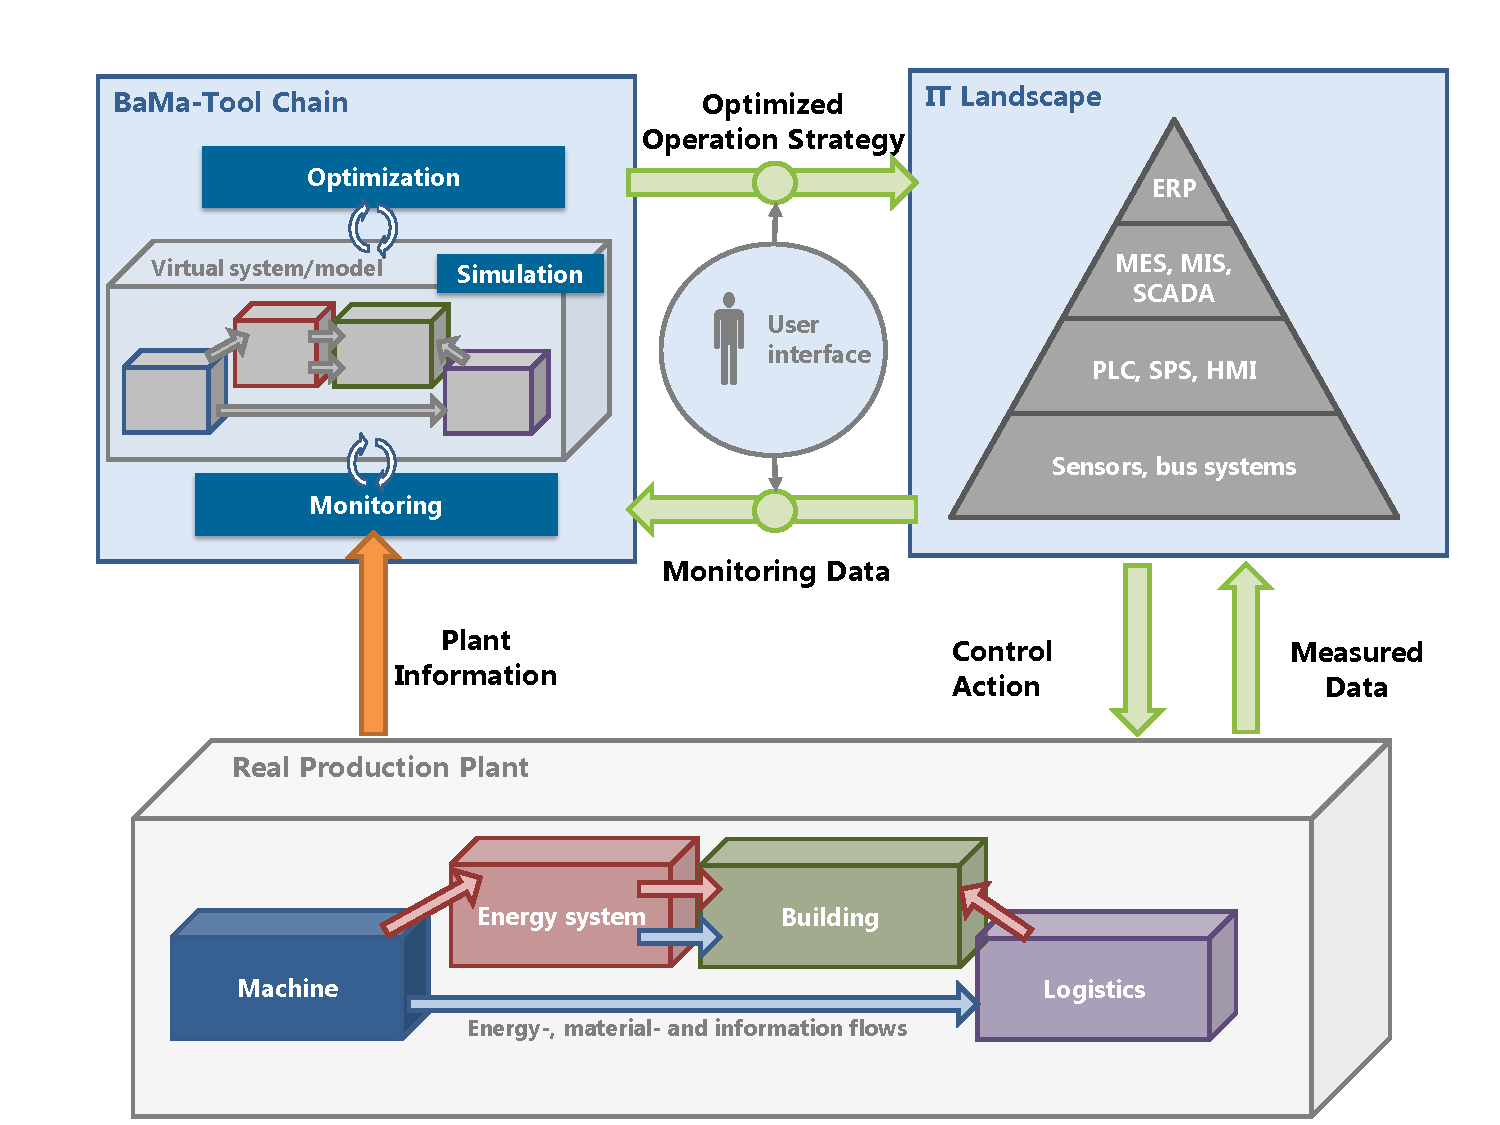
\includegraphics[width=0.5\textwidth]{figures/Architecture_new}
	\caption{BaMa Architecture}
	\label{FIG_Architecture}
\end{figure}
Figure \ref{FIG_Architecture} shows the relationships between the proposed tool chain, the production site and IT landscape. A conventional IT landscape is the link between BaMa tool chain and the production site. It transmits all relevant data to the BaMa Monitoring module. Using monitoring data and other qualitative and quantitative information about the plant under consideration, a simulation model of the production site is established. This virtual twin of the real world stands at the core of the BaMa tool chain. Together with an optimization module, this can be used to generate optimized operation strategies. Those are reviewed by a human supervisor. Afterwards, the operation strategy can be handed over to the respective layer in the IT landscape. The proposed and reviewed operation strategy is processed and  control commands can be sent to the respective system. In order for BaMa to unfold its full optimization potential, this process needs to be carried out and executed on a regular basis. Therefore, a high integration into existing automation systems is necessary. \\
For the chillers under consideration in this paper, the following steps where carried out:
\begin{itemize}
	\item{Monitoring: Structural plant information,\linebreak sensor data from an existing SCADA system corresponding to measurements of temperatures, electrical power and heat connected with chillers and cooling towers as well as other information from the IT-landscape (e.g. from enterprise resource planning or manufacturing execution systems) was used to build a simulation model. According to \cite{monostori_cyber-physical_2014}, this intensive connection of embedded systems (sensors) with ongoing processes is among the main characteristics of CPS.}
	\item{Simulation: Measured data and plant information are used to build a virtual representation of the production site. The resulting model allows forecasting of the overall energy demand based on a set of input parameters. It implemented using AMESIM\footnote{\url{https://www.plm.automation.siemens.com/de_at/products/lms/imagine-lab/amesim/}}, a simulation environment and integrated into the existing SCADA system on premise.}
	\item{Optimization: The evaluation of the results of repeated simulations enables an optimization framework to find beneficial operation plans for the virtual plant. Optimization targets in this case where the electrical power input as well as the additionally needed heat from external sources. Other potential targets might be machine-operating hours.}
\end{itemize}
As mentioned, within the tool chain a "virtual twin" of the real production plant (i.e. a model) is used to predict the behaviour of the physical system. The potential modelling effort is considerable and needs to be minimized in order to make BaMa a feasible and applicable tool for companies. To address this, the cube concept is introduced and will be explained in the following section.
\subsection{Modelling Approach}
\begin{figure}
	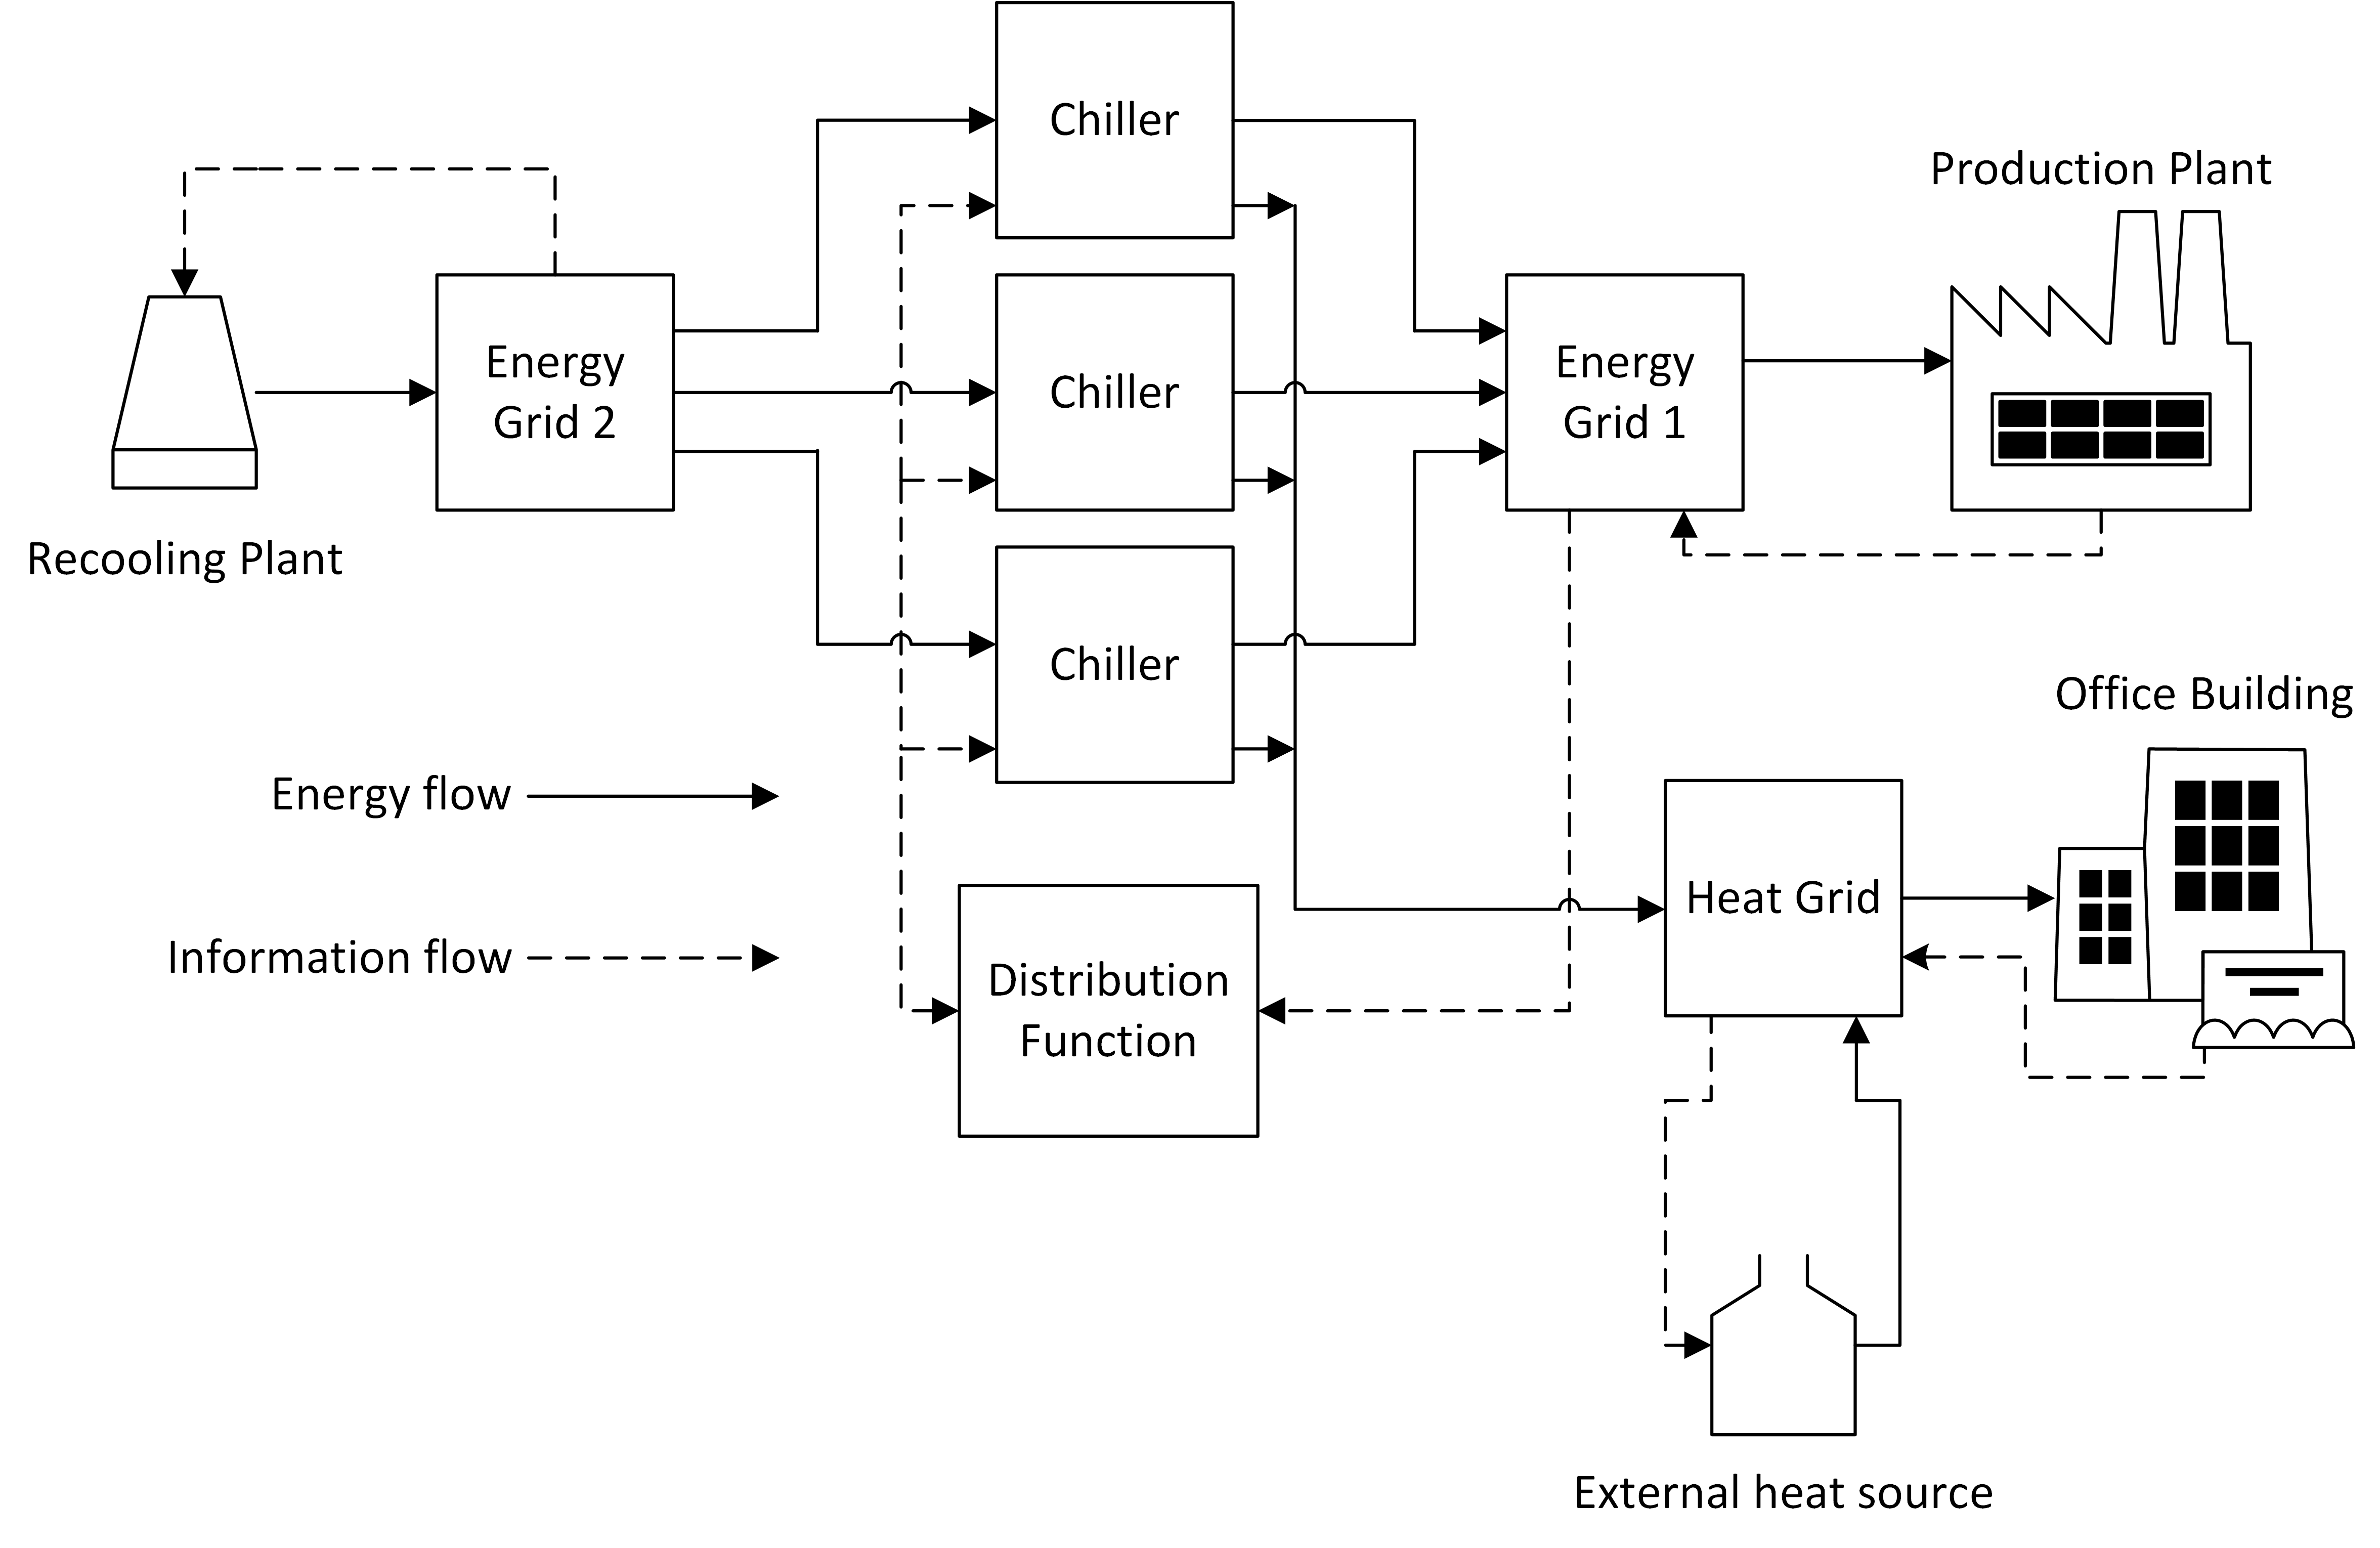
\includegraphics[width=0.5\textwidth]{figures/modelstructure}
	\caption{BaMa Architecture}
	\label{FIG_Model}
\end{figure}
Each production site needs to be modelled individually in order to be able to generate valid optimization strategies. For BaMa to be feasible despite this issue, a high degree of model re-usability must be achieved. \cite{Balci2012,Setavoraphan2008} suggest decomposition at model design level when dealing with simulations of comparable scope.\\
Object-oriented software engineering follows similar design principles. Entity classes and their possible interaction are defined using entity-relationship models (ERM) thus providing a certain kind of standardization. The inner behaviour of those entities is encapsulated and hidden from the outside. The only interactions with the surroundings happens via interfaces. As a consequence, entities can be removed and replaced without impeding  the overall model \cite{Schatten2010}.
The decomposition into smaller parts following the divide-and-conquer principle makes it possible to reuse existing models by describing relevant subsystems of the plant as instances of predefined entity classes. In the BaMa context, those smaller parts are called "cubes". They have defined interfaces and boundaries have proven useful in the modelling of production facilities.
In figure \ref{FIG_Cube}, an example cube is depicted. It represents a generic model of an industrial chiller. As can be seen, there are generally two different kinds of interfaces a cube can have: energy and information flows. Using these interfaces, a chiller can be connected with similar models such as energy nets, cooling towers or other compatible cubes. Based on the model proposed by \cite{Hydeman2002}, the inner parameters are used to define how the inputs and outputs of the model are connected and therefore determine how a given chiller instance behaves at different set points. Those parameters need to be estimated on the basis of monitoring and/or specification data. This process will be described in the following section.
\begin{figure}
	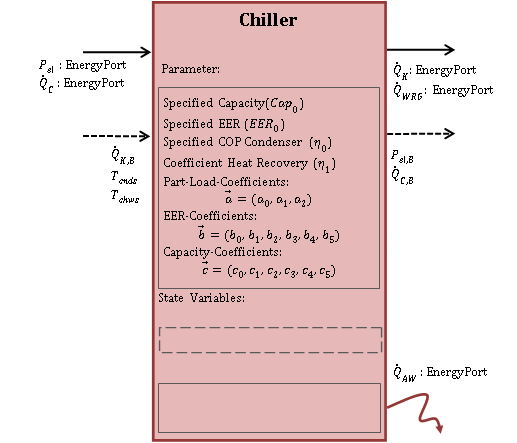
\includegraphics[width=0.5\textwidth]{figures/Chiller_Cube}
	\caption{Chiller Cube}
	\label{FIG_Cube}
\end{figure}
\section{Use Case}
As stated earlier, the optimization of the operation of an industrial chiller network is at the central of this paper. The system under investigation is depicted in figure \ref{FIG_Model}. In total, twelve chillers with electrical power input rates between 300 and 500kW where investigated. Apart from producing chilled water, some of the chillers are also used to aid the heating network using heat recovery. Those chillers capable of providing heat to the HVAC system have a significantly worse COP then those without this capability. The goal of this use case was to identify operating strategies for the chillers based on given heating and cooling demands from external sinks (production plant and office building). In accordance with the BaMa method, monitoring data was used to parametrize the models. They then where implemented using a simulation tool-chain. Lastly, an optimization algorithm was applied. 

\subsection{Model Parametrization}
An approach to identify the chillers model coefficients by using collected monitoring data was chosen based on \cite{Monfet}. Data including the electric power input (P\textsubscript{e}) and the evaporator load (Q\textsubscript{e}) got measured from eight chillers, and additionally the chilled water supply temperature (T\textsubscript{chws}) and the temperature leaving the condenser (T\textsubscript{cnds}) from four chillers were monitored over a time period of at least one month (Table 1). The available data was collected every 30 seconds from each chiller. In order to improve the identification (parameter estimation) process, outliers and incomplete data where removed from the dataset. 

\begin{table}
	\caption{monitored chillers data}
	\begin{tabular*}{\hsize}{@{\extracolsep{\fill}}@{\hskip6pt}lll@{\hskip6pt}lll@{\hskip6pt}lll@{\hskip6pt}lll@{\hskip6pt}lll@{\hskip6pt}}
		\toprule
		Chiller & P\textsubscript{e} & Q\textsubscript{e} & T\textsubscript{chws} & T\textsubscript{cnds} & \multicolumn{2}{l}{data set size}\\
			& & & & & without filter & with filter\\
		\colrule
		B24\_1 &   X &  X &  & & 919865 & 919757 \\
		B24\_2 &   X &  X &  & & 1124472 & 1124415 \\
		B24\_3 &   X &  X &  & & 1125003 & 1124808 \\
		B24\_4 &   X &  X &  & & 1125671 & 1125611 \\
		B24\_5 &   X &  X &  & & 915289 & 915143 \\
		B24\_6 &   X &  X &  & & 1134663 & 1134474 \\
		B24\_7 &   X &  X &  & & 1127933 & 844476 \\
		B24a\_1 &   X &  X & X & X & 678718 & 583815 \\
		B24a\_2 &   X &  X & X & X & 679007 & 587077 \\
		B24a\_3 &   X &  X & X & X & 679250 & 591193 \\
		B24a\_4 &   X &  X & X & X & 679451 & 556556 \\
		B24a\_5 &   X &  X & X & X & 103660 & 74159 \\
		\botrule
		\label{TAB_Data}
	\end{tabular*}
\end{table}

Three types of filters where applied to the data:
\begin{itemize}
	\item Incomplete Data: Data, where one of the measured attributes was missing
	\item Outliers: Data, where measurements lay beyond threefold the standard deviation (equation \ref{EQU_STD})
	\item Physical soundness: Were temperatures where measured, any data containing temperature signals T\textsubscript{cnds} and T\textsubscript{chws} outside of the limits declared in table \ref{TAB_Limits} 
\end{itemize}
Datasets that fulfil at least one of the filter criteria where removed before the fitting process.  

\begin{table}
	\caption{Temperature limits}
	\begin{tabular*}{\hsize}{@{\extracolsep{\fill}}@{\hskip6pt}lll@{\hskip6pt}lll@{\hskip6pt}}
		\toprule
		& T\textsubscript{cnds} ({\it{\degree C}}) & T\textsubscript{chws} ({\it{\degree C}}) \\
		\colrule
		Upper limit & 30 & 15\\
		Lower limit & 15 & 4\\
		\botrule
		\label{TAB_Limits}
	\end{tabular*}
\end{table}

\begin{equation}
\begin{array}{@{}lcl}
\displaystyle y_i &<& \displaystyle y_{mean} - 3 \cdot \sigma \\[6pt]
\displaystyle y_i &>& \displaystyle y_{mean} + 3 \cdot \sigma \\[6pt]
\end{array}\vspace*{-12pt}
\label{EQU_STD}
\end{equation}

The result of the filtering process is shown in Table \ref{TAB_Data}. Up to 28\% of the original data had to be removed due to the filter criteria.  
For parametrization, the filtered data was split into a training and a validation dataset, with a split ratio of 0.9 by random selection. For the machines with measured data of the power input (P\textsubscript{e}), the evaporator load (Q\textsubscript{e}), the chilled water supply temperature (T\textsubscript{chws}) and the temperature leaving the condenser (T\textsubscript{cnds}) the approach described by \cite{Monfet} was used. For the other chillers, where there was no monitored data of the temperatures, a simpler model was applied by setting the temperature-depending coefficients of the model to zero. 
The relative RMSE, for the dataset with and without filter, is shown in Equation \ref{EQU_RMSE}. It is apparent that for some machines the model accuracy is significant increased by preprocessing.

\begin{equation}
\begin{array}{@{}lcl}

\displaystyle 
RMSE_{rel} &=& 
\displaystyle 
\frac
{\sqrt[]{\sum_{i=1}^n \left(y_{i,predicted} - y_i\right)^2}}
{\sum_{i=1}^n y_i}
\cdot 100
\\[6pt]

\end{array}\vspace*{-12pt}
\label{EQU_RMSE}
\end{equation}

\begin{table}
	\caption{Prediction errors}
	\begin{tabular*}{\hsize}{@{\extracolsep{\fill}}@{\hskip6pt}lll@{\hskip6pt}lll@{\hskip6pt}lll@{\hskip6pt}lll@{\hskip6pt}lll@{\hskip6pt}lll@{\hskip6pt}}
		\toprule
		& \multicolumn{4}{c}{RMSE\textsubscript{rel}} \\
		& \multicolumn{2}{l}{with filter} & \multicolumn{2}{l}{without filter} & used for Optimization\\
		Chiller & P\textsubscript{e} & Q\textsubscript{con} & P\textsubscript{e} & Q\textsubscript{con} & \\
		\colrule
		B24\_1 & 13.6 & 65.1 & 13.4 & 65.2 & X \\
		B24\_2 & 17.2 & 4.5 & 16.7 & 4.4 & X \\
		B24\_3 & 4.7 &  10.0  & 4.9 & 10.4 & X \\
		B24\_4 & 26.9 &  21.2 & 27.0 & 20.4 & X \\
		B24\_5 & 38.5 &  48.6 & 37.3 & 48.6 & X \\
		B24\_6 & 178.3 &  722.2 & 178.0 & 722.7 &  \\
		B24\_7 & 126.1 &  136.2 & 189.6 & 100.9 &  \\
		B24a\_1 & 28.8 & 69.1 & 23.3 & 64.3 & X \\
		B24a\_2 & 10.3 & 3.9 & 1109.2 & 181.2 & X \\
		B24a\_3 & 4.4 & 8.4 & 6.3 & 8.5 & X \\
		B24a\_4 & 11.8 & 29.7 & 10.9 & 30.1 & X \\
		B24a\_5 & 179.5 & 432.2 & 252.2 & 318.6 &  \\
		\botrule
		\label{TAB_Errors}
	\end{tabular*}
\end{table}

Due to the fact that some models describe the associated chillers with a large RMSE\textsubscript{rel}, these were not taken into account for the subsequent optimization.

\subsection{Model Implementation}

In this section the implementation of the model in AMESIM is described. Even though some predefined models are provided for, the built-in libraries of did not meet the requirements of the system, so both the models for chillers and energy grids had to be implemented from scratch. Regarding the signal routing between the models however, it was possible to use standard components. Logically, the simulation input is the power demand (cooling and heating) from the production building. This requirement is sent to the energy grid as an information flow. The energy grid fulfils the requirement by sending cooling power to the production plant. As a consequence, the energy level in the grid changes. This change is described using the following equation:

\begin{equation}
\begin{array}{@{}lcl}

\displaystyle 
\frac{\partial E}{\partial t} &=& 
\displaystyle 
\frac
{1}
{C}
\cdot \left
(\dot{Q}_{producer} - \dot{Q}_{consumer}\right)
\\[6pt]

\end{array}\vspace*{-12pt}
\end{equation}

C is the heat capacity of the grid. It depends on the parameters mass m in the grid and the specific heat capacity c\textsubscript{p}:

\begin{equation}
\begin{array}{@{}lcl}

\displaystyle 
C &=& 
\displaystyle 
m \cdot c_p
\\[6pt]

\end{array}\vspace*{-12pt}
\end{equation}

Using the current energy level E in the grid, the temperature of the fluid can be calculated:

\begin{equation}
\begin{array}{@{}lcl}

\displaystyle 
T &=& 
\displaystyle 
\frac{E}
{m \cdot c_p}
+ T_0
\\[6pt]

\end{array}\vspace*{-12pt}
\end{equation}

The internal variable E is the controlled variable of the grid. It is controlled by a PI-Controller. Energy grid 1 demands cooling power based on a distribution function. This function splits the demand in several parts and sends it to the respective chillers. This is done by comparing two variables: the required heat flow Q\textsubscript{e,r} from the energy grid and the currently produced heat flow Q\textsubscript{e} from the chillers. If less cooling power is produced than consumed, the distribution function starts the next chiller. The sequence in which the chillers are started is defined in the priority list. 

The chiller submodel receives the following energy flows: P\textsubscript{el}, Q\textsubscript{c} as an external input and Q\textsubscript{e}, Q\textsubscript{hr} as an external output. The information flows used are: the temperatures in energy grid 1 T\textsubscript{chws} and the temperature in energy grid 2 T\textsubscript{cnds}. The recovered heat flow Q\textsubscript{hr} is fed into the heat grid, which provides the office buildings (see figure 1) with a heat flow.

Q\textsubscript{hr} depends on the evaporator loading conditions. That is why it is calculated using Q\textsubscript{e}. The heat recovery efficiency coefficient  $ \eta\textsubscript{1} $ was determined by linear regression analysis and the method of least squares.

\begin{equation}
\begin{array}{@{}lcl}
\displaystyle 

\dot{Q}_{hr} &=& \eta_{1}\dot{Q}_{e} 

\\[6pt]
\end{array}\vspace*{-12pt}
\end{equation}

By using the heat recovery systems of the chillers, the heat energy required from external sources Q\textsubscript{h,net} is reduced. If the heat recovery systems provide more heat energy, than consumed, no heat from external sources is needed and Q\textsubscript{h,net}=0:

\begin{equation}
\begin{array}{@{}lcl}
\displaystyle 

\dot{Q}_{h,net} &=&  
\left\{ \begin{array}{lcl}
\dot{Q}_{h,gross} - \dot{Q}_{hr} & &,\ if\ \dot{Q}_{h,gross} > \dot{Q}_{hr} \\ 
0 & &,\ if\ \dot{Q}_{h,gross} < \dot{Q}_{hr}
\end{array}\right.

\\[6pt]
\end{array}\vspace*{-12pt}
\end{equation}

To emit the heat of the chillers to the environment, cooling towers are used. Those where modelled by just applying a maximum possible heat flow Q\textsubscript{cmax} to the environment. If the required cooling energy flow Q\textsubscript{c} from the chillers is higher than Q\textsubscript{cmax}, not enough heat can be emitted to the environment and the temperature Tcnds in energy grid 2 rises. This influences CAPFT and EIRFT in the chillers as shown above.
The same effects occur when the requirement of cooling power Q\textsubscript{e,r} exceeds the maximum possible heat flow Q\textsubscript{e} from the chillers. The energy level in grid 1 changes and the temperature T\textsubscript{chws} rises. The simulation considers this dynamic behaviour of the grids and the effects on the chillers.

\subsection{Optimization}
Based on the analysis of the model errors, 9 chillers were selected for optimization (Table \ref{TAB_Errors}). The scenarios considered where derived from typical production days. Throughout those, the power demands fluctuate and chillers need to be switched on and off. A switch-on sequence, which is modelled as a priority list, determines the order in which this happens. Consequently, the optimization problem has nine degrees of freedom and therefore 9! ≈ 3.6E9 potential solutions. A genetic algorithm was chosen to find a time-efficient optimum.
An example for a vector is given here:

\begin{equation}
\begin{array}{@{}lcl}

\displaystyle 
\vec{p} &=& 
\displaystyle 
\left(8,2,4,9,6,7,5,3,1\right)
\\[6pt]

\end{array}\vspace*{-12pt}
\end{equation}

The vector can be read as follows: machine 8 is switched on first, then machine 2, then machine 4 and so on. Every entry in the priority vector is a natural number in the range from 1 to 9 and is unique.A built in genetic optimization algorithm was chosen for this problem. This algorithm however does not support vectors as a regular input. Therefore, a list of all possible vectors, was defined. The optimizer then modified an integer representing a vector.\\
Another core part of the optimization is the fitness function (equation \ref{EQU_Fitness}). Based on this, the result of each simulation run is evaluated. In this function, relevant parts of the simulation results are aggregated using corresponding weights to result in a fitness value which is minimised by the optimization algorithm.

\begin{equation}
\begin{array}{@{}lcl}

\displaystyle 
f &=& 
\displaystyle 
\omega_{1}P_{el,r} + \omega_{2}Q_{h,net}
\\[6pt]

\end{array}\vspace*{-12pt}
\label{EQU_Fitness}
\end{equation}

The fitness function consists of two main parts: the first part is weighted with $ \omega_{1} $ and considers the electrical energy consumption P\textsubscript{el,r}. The second part is weighted with $ \omega_{2} $ and considers the heat energy consumption from external sources Q\textsubscript{h,net}. The heat energy consumption from external sources is calculated as the difference between the required heat energy and the heat provided by the chillers with heat recovery system (see section model implementation).
By setting the weight factors, different goals can be pursued. To perform an optimization of the energy consumption in the scenario, all factors can be set to 1. Then the optimizer directly minimizes the consumed energy in the scenario. Another goal could be the optimization of the costs. If both weighting factors are set to the energy prices for electricity and heat, the costs can be calculated directly from the fitness value and the optimizer minimizes the costs. Another use case is to reduce the impact on the environment by minimizing the CO\textsubscript{2}-Emissions. In order to do so however, detailed information about the sources of electric and heat energy is required. The weighting factors can be set depending on the emitted CO\textsubscript{2} by producing 1 kWh electric energy and 1 kWh heat energy.
The performance of the optimization process highly depends on the workload of the chillers. If the workload is high, a high number of chillers is running and the impact of the priority vector on the performance is reduced. If the workload is lower, there are more different switch-on sequences, so the optimizer has more degrees of freedom to reduce the fitness value. To evaluate the performance of the optimization process, scenarios with high and low workload conditions are investigated separately (table \ref{TAB_Scenarios}).
In the first scenario, heat energy requirement weighting factor is set to 0. The electric energy consumption P\textsubscript{el,r},rlb is the only variable effecting the fitness value. In the second scenario, the heat energy requirement weighting factor is set to 1. In this case, an optimization of the total energy consumption (electricity and heat) is performed. An overview of the used weighting and cost factors is given in table \ref{TAB_Scenarios}.

\begin{table}[t]
	\caption{weight factors and part load ratio for the scenarios}
	\begin{tabular*}{\hsize}{@{\extracolsep{\fill}}@{\hskip6pt}lll@{\hskip6pt}lll@{\hskip6pt}lll@{\hskip6pt}
			lll@{\hskip6pt}lll@{\hskip6pt}lll@{\hskip6pt}lll@{\hskip6pt}lll@{\hskip6pt}lll@{\hskip6pt}}
		\toprule
		scen. & \multicolumn{2}{l}{optimized}  & 
		T\textsubscript{chws}  & T\textsubscript{cnds} 
		& Q\textsubscript{e,r} & PLR & Q\textsubscript{h,gross} 
		& $\omega\textsubscript{1} $ & $\omega\textsubscript{2} $\\
		& \multicolumn{2}{l}{values} & ({\it{\degree C}}) & ({\it{\degree C}})& ({\it{kWh}}) &  ({\it{\%}}) & ({\it{kWh}})\\
		&  P\textsubscript{el,r} &  Q\textsubscript{h,net}\\
		\colrule
		1 & X & & 7.8 & 25.1 & 4.7E5 & 84.4 & 61375 & 1 & 0\\
		2 & X & & 7.2 & 24.3 & 2.0E5 & 35.9 & 86722 & 1 & 0\\
		3 & X & X & 7.2 & 25.1 & 4.7E5 & 84.4 & 61375 & 1 & 1\\
		4 & X & X & 7.8 & 24.3 & 2.0E5 & 35.9 & 86722 & 1 & 1\\
		\botrule
		\label{TAB_Scenarios}
	\end{tabular*}
\end{table}

Table \ref{TAB_OptResults} shows the electric energy consumption of a simulated optimized priority vector compared to measured data. A reduction can be achieved with both workload (PLR) conditions. The reduction ratio highly depends on the workload. A higher workload leads to less optimization potential. 
Scenario 3 and 4 are the same with the heat recovery systems included in the fitness function. So there are two main variables that effect the fitness value: P\textsuperscript{el,r} and Q\textsubscript{h,net}. Because of the influence of Q\textsubscript{h,net} to the fitness value, the reduction ratio is even higher, than without heat recovery. The results also depend on the operation strategy of the chillers in operation while the measured data sets were recorded.

\begin{table}[t]
	\caption{Optimization performance}
	\begin{tabular*}{\hsize}{@{\extracolsep{\fill}}@{\hskip6pt}lll@{\hskip6pt}lll@{\hskip6pt}lll@{\hskip6pt}
			lll@{\hskip6pt}lll@{\hskip6pt}lll@{\hskip6pt}lll@{\hskip6pt}lll@{\hskip6pt}lll@{\hskip6pt}}
		\toprule
		scen. & PLR & \multicolumn{2}{l}{energy use ({\it{kWh}})}  & reduction \\
		& ({\it{\%}}) & with optimization & without optimization & ({\it{\%}})\\

		\colrule
		1 & 84.4 & 104592 & 89038 & 14.87\\
		2 & 35.9 & 53958 & 35094 & 34.96\\
		3 & 84.4 & 115672 & 90295 & 21.94\\
		4 & 35.9 & 70351 & 41473 & 41.05\\

		\botrule
		\label{TAB_OptResults}
	\end{tabular*}
\end{table}

\section{Conclusion}
In this article we presented a novel method called BaMa Method which was applied to the problem of optimal selection of industrial chillers. This was done using simulation models of the underlying system, which where derived from monitoring data. Different target functions where tested in order to reflect varying management targets. This goes beyond what similar 
Regarding the next steps, further work will be done on the improvement of model quality. Using the current models, still an overall error of up to 28\% has to be expected in the worst case. Also the optimization time will be improved by selecting more intelligent implementations.
Both, the modelling quality and the optimization time are due to the chosen software environment AMESIM, which prevented the use of more sophisticated modelling techniques.
\bibliography{Data_based_optimization}   % name your BibTeX data base
\bibliographystyle{elsarticle-num}      % mathematics and physical sciences
\end{document}

%%
%% End of file `procs-template.tex'.
